\section{Zielsetzung}
Ziel des Versuches ist es einerseits die Charakteristik eines Geiger-Müller-Zählrohres und andererseits die Totzeit desselben
mittels unterschiedlicher Methoden zu bestimmen. 
\section{Theorie}
\label{sec:Theorie}
\subsection{Funktionsweise eines Geiger-Müller-Zählrohres}
Mit einem Geiger-Müller-Zählrohr lässt sich ionisierte+ Strahlung messen. Dabei tritt ein geladenes $\symup{\alpha}$- oder $\symup{\beta}$-
Teilchen in das Zählrohr ein, ionisieren die Atome des Gases, sodass die herausgelösten Elektronen einen Impuls auslösen.
Das Zählrohr besteht dabei aus einem Aufbau, wie er in \autoref{fig:zaehlrohr}
schematisch dargestellt ist. Es ist mit einem Gasgemisch aus Argon und Ethylalkohol. Durch Anlegen einer Spannung zwischen dem Anodendraht und
der Zylinderkathode erfahren geladene Teilchen eine Beschleunigung zum Draht hin. Diese kann für beliebig kleine Radien des Drahtes
$r_{\symup{a}}$ zum Draht hin beliebig groß werden.
\begin{figure}
    \centering
    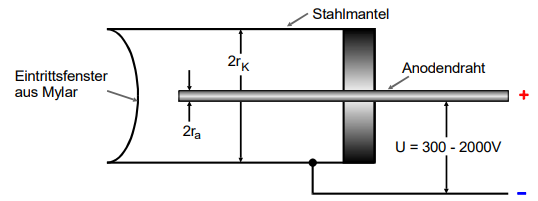
\includegraphics[width=0.9\textwidth]{content/aufbau.png}
    \caption{Skizzenhafter Querschnitt eines Zählrohres.}
    \label{fig:zaehlrohr}
\end{figure}
Wenn nun ein geladenes Teilchen (beispielsweise $\symup{\alpha}$- oder $\symup{\beta}$-Teilchen) in das Zählrohr eintritt, bewegt es sich so 
lange durch das Gas, bis die Energie des Teilchens durch Ionisationsprozesse aufgebraucht ist. Die Anzahl der herausgelösten Elektronen
ist dabei proportional zur Energie des einfallenden Teilchens.
Das Verhalten des Zählrohres nach dieser Primärionisation hängt dabei von der angelegten Spannung ab. Dies ist in \autoref{fig:spannung}
veranschaulicht. Zu sehen sind dabei 5 Spannungsbereiche. In Bereich I erreichen erst nur wenige Elektronen den Draht, da sie zuvor
wieder rekombinieren. Bei steigender Spannung steigt auch die Anzahl der den Draht erreichenden Elektronen stark an. Bereits in Zone II
erreichen praktisch alle Elektronen den Draht und es ist ein Ionisationsstrom, welcher proportional zur Energie der Elektronen ist, messbar.
Dies wird auch als Ionisationskammer bezeichnet und ist, da die messbaren Ströme sehr gering sind, nur bei hohen Strahlintensitäten einsetzbar.
Bei weiterer Erhöhung der Spannung, wie in Bereich III zu sehen, erreichen die Elektronen solche Energien, dass sie ihrerseits sogenannte
Stoßionisationen durchführen können, wobei die dadurch herausgelösten Elektronen ebenfalls bei hinreichend hoher Spannung Ionisationen
auslösen können. Da die Anzahl der Elektronen so sehr stark ("lawinenartig") zunimmt, wird dies Townsend-Lawine genannt. Da die
Ladung pro einfallendes Teilchen nun so groß ist, dass sie als Ladungsimpuls gemessen werden kann, und sie immer noch proportional zur
Energie ist, lässt sich eine direkte Energiemessung durchführen.
Der Arbeitsbereich des Geiger-Müller-Zählrohres liegt allerdings bei noch höheren Spannungen im Bereich IV. Hier breiten
sich die Elektronenlawinen auf der gesamten Länge des Anodendrahtes aus, da diese im gesamten Zählrohrvolumen
enstehen. Das kommt dadurch zustande, dass während der primären Elektronenlawine Photonen im UV-Bereich enstehen, welche sich auch senkrecht
zum elektrischen Feld bewegen können, da sie Ladungsfrei sind. Sie stellen daher den Ausgangspunkt weiterer Elektronenlawinen dar.
Dieser Bereich wird Auslösebereich genannt und beginnt in \autoref{fig:spannung} in etwa dort wo sich die Kurven von $\symup{\alpha}$- und
$\symup{\beta}$- Strahlung schneiden.
In diesem Bereich lässt sich das Zählrohr allerdings nur noch zur Intensitätsmessung nutzen.
\begin{figure}
    \centering
    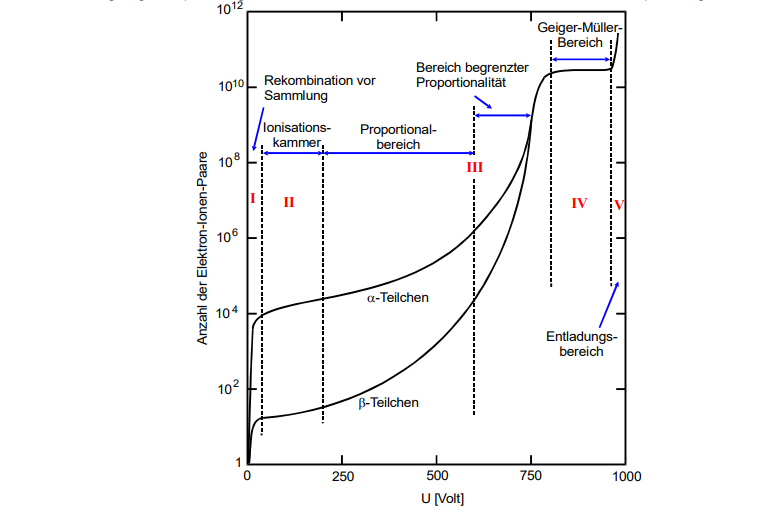
\includegraphics[width=0.9\textwidth]{content/bereich.png}
    \caption{Anzahl der erzeugten Elektron-Ion-Paare als Funktion der Spannung U bei einem Proportionalzählrohr.}
    \label{fig:spannung}
\end{figure}
\subsection{Totzeit und Nachentladungen}
Nach der Ionisation bewegen sich die Elektronen schnell zum Anodendraht, während die positiven Ionen aufgrund ihrer größeren Masse
vergleichsweise länger zum Kathodenzylinder benötigen. Dadurch entsteht zwischenzeitlich eine positve Raumladung im Zählrohr, welche
so hoch ist, dass während dieser Zeit keine Stoßionisationen möglich sind und eintreffende Teilchen dadurch nicht registriert werden können.
Diese Zeit wird als Totzeit $T$ bezeichnet. Die gemessenen Ladungsimpulse erreichen aber erst dann wieder ihre volle Höhe, wenn die Ionen
vollständig neutralisiert sind. Die dazu benötigte Zeit wird als Erholungszeit $T_{\symup{E}}$ bezeichnet, wie in \autoref{fig:tot} zu
sehen. Des Weiteren sind die Ionen in der Lage Elektronen aus der Kathode auszuschlagen, was dazu führt, dass nach der Messung eines Teilchens
weitere Impulse enstehen. Diese zusätzlichen Impulse werden als Nachentladungen bezeichnet. Ihr zeitlicher Abstand von dem tatsächlichen Impuls
$T_{\symup{L}}$ ist in der Regel länger als die Totzeit $T$, weshalb diese Nebeneffekte unerwünscht sind. Die Häufigkeit dieser Ereignisse
wird dadurch gesenkt, dass ein Alkoholgas zugefügt wird. Dabei versetzt die Energie der Ionen die Alkoholmoleküle in
Schwingung, wodurch die Energie zu gering wird um Elektronen aus der Kathode zu schlagen. Das Zählrohr wird somit nur noch durch neue einfallende
Teilchen ausgelöst.
\begin{figure}
    \centering
    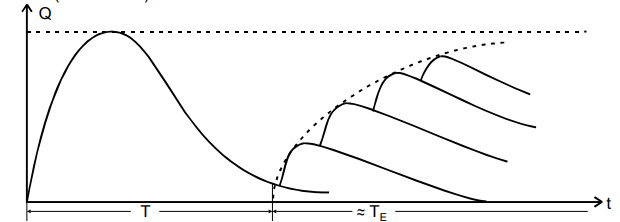
\includegraphics[width=0.9\textwidth]{content/totzeit.png}
    \caption{Totzeit und Erholungszeit in einem Ladungs-Zeit-Diagramm.}
    \label{fig:tot}
\end{figure}
\subsection{Charakteristik des Geiger-Müller-Zählrohres}
Die Charakteristik eines Zählrohres beschreibt die Anzahl der registrierten Teilchen $N$, welche gegen die Spannung $U$ aufgetragen wird.
Dies ist in \autoref{fig:char} veranschaulicht. Zu sehen ist, dass der Auslösebereich bei einer Spannung $U_{\symup{E}}$ beginnt und dort
annähernd konstant, was als Plateau bezeichnet wird. Da es sich in der Realität nicht um ein ideales Zählrohr handelt, hat das Plateau
eine leichte Steigung. Diese wird durch einige Nachentladungen hervorgerufen, welche trotz des Alkoholgases enstehen können. Dabei
ist die Qualität eines Zählrohres umso höher, je geringer diese Steigung ist. Am Ende des Plateaus nimmt die Teilchenzahl stark zu, hier
führt das Gas selbständig Entaldungen durch.
In diesem Spannungsbereich würde das Zählrohr schnell zerstört werden.
\begin{figure}
    \centering
    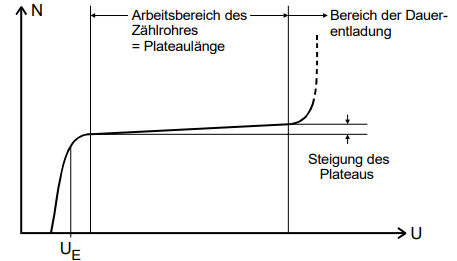
\includegraphics[width=0.9\textwidth]{content/charakteristik.png}
    \caption{Anzahl der Teilchen gegen die Spannung mit Charakteristik.}
    \label{fig:char}
\end{figure}
\subsection{Bestimmung der Totzeit mittels der Zwei-Quellen-Methode}
Zur Bestimmung der Totzeit kann die sogenannte Zwei-Quellen Methode herangezogen werden. Hierbei wird zunächst über einen festen
Zeitraum und bei einer festen Spannung, bei der die Strahlintensität hoch ist, die Zählrate $N_1$ einer Quelle bestimmt. Anschließend wird eine
zweite Quelle im selben Abstand vom Zählrohr hinzugefügt und die Zählrate über den selben Zeitraum $N_{1+2}$ aufgenommen. In einem letzten
Schritt wird die erste Quelle entfernt und nur die Zählrate $N_2$ der zweiten Quelle bestimmt. Die Totzeit ermittelt sich dann zu
\begin{equation}
\label{eqn:totzeit}
T \approx \frac{N_1 + N_2 - N_{1+2}}{"\cdot N_1 N_2}.
\end{equation}
